\section{Habib Abdul Rasyid(1174002)}
\subsection{Instalasi Map Server}
\begin{enumerate}
    \item Download dulu ms4w nya di web resminya yaitu ms4w.com/download.html
    \hfill\break
    \begin{figure}[H]
		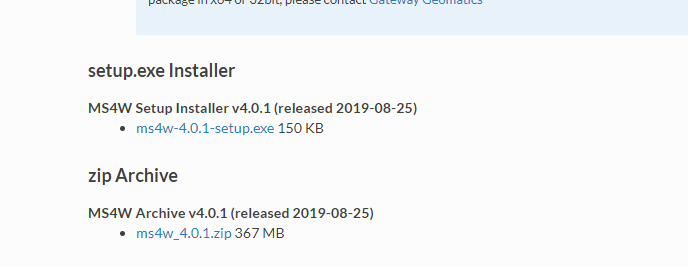
\includegraphics[width=4cm]{figures/1174002/4/1.png}
		\centering
		\caption{Download File MS4W}
    \end{figure}
    \hfill\break

    \item Setelah di download, bisa langsung melakukan Instalasi. Untuk versi windows bisa saya sarankan mendownload yang .exe agar lebih mudah saat instalasi.
    \item Instalasi Menggunakan Option Full Install

\end{enumerate}


\subsection{Konfigurasi Map Server}
Jika telah selesai melakukan instalasi kita akan melakukan konfigurasi
\begin{enumerate}
  \item Buka folder ms4w. Masuk ke folder apache
  \hfill\break
    \begin{figure}[H]
		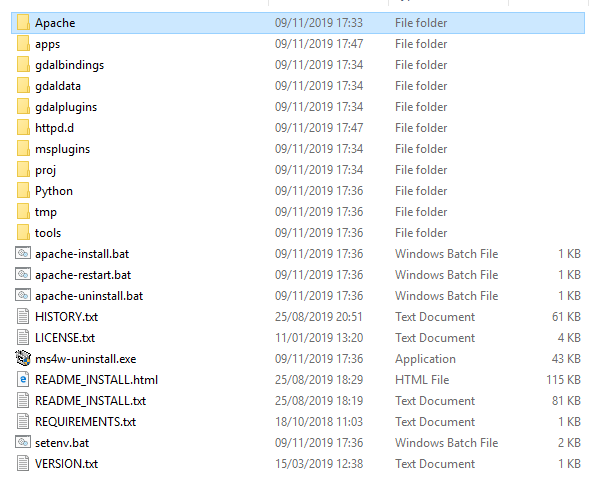
\includegraphics[width=4cm]{figures/1174002/4/3.png}
		\centering
		\caption{Isi Folder apache}
    \end{figure}


  \item Masuk ke folder conf
  \hfill\break
    \begin{figure}[H]
		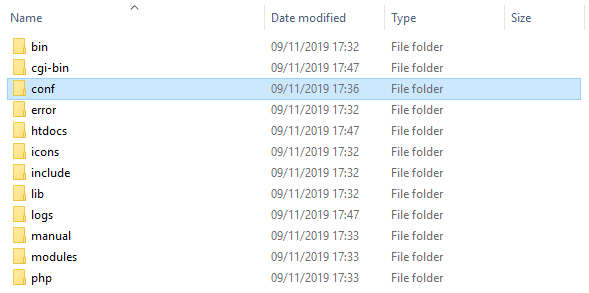
\includegraphics[width=4cm]{figures/1174002/4/4.png}
		\centering
		\caption{Folder conf}
    \end{figure}
  \item Masuk ke folder conf
  \hfill\break
    \begin{figure}[H]
		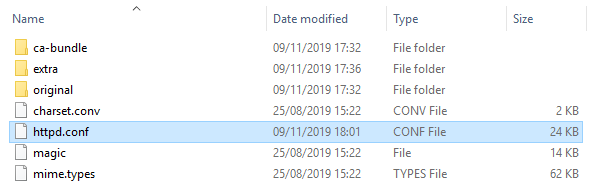
\includegraphics[width=4cm]{figures/1174002/4/5.png}
		\centering
		\caption{Isi Folder Conf}
    \end{figure}

  \item Buka file httpd.conf dan ubah listen port nya. Karena dikomputer saya port 80 digunakan untuk webserver, port ini juga bisa d setting saat proses instalasi sebelumnya.
  \hfill\break
    \begin{figure}[H]
		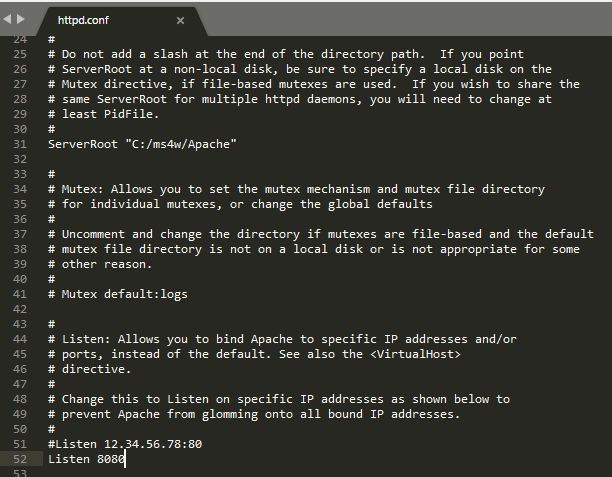
\includegraphics[width=4cm]{figures/1174002/4/6.png}
		\centering
		\caption{Listen port}
    \end{figure}

  \item Kemudian kita jalankan servisnya, dengan menggunakan tombol windows + r dan ketikan services.msc
  \hfill\break
    \begin{figure}[H]
		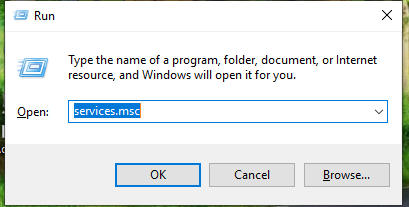
\includegraphics[width=4cm]{figures/1174002/4/7.png}
		\centering
		\caption{Mengakses Halaman Service}
    \end{figure}

  \item Cari servis untuk Apache MS4W Web Server
    \begin{figure}[H]
		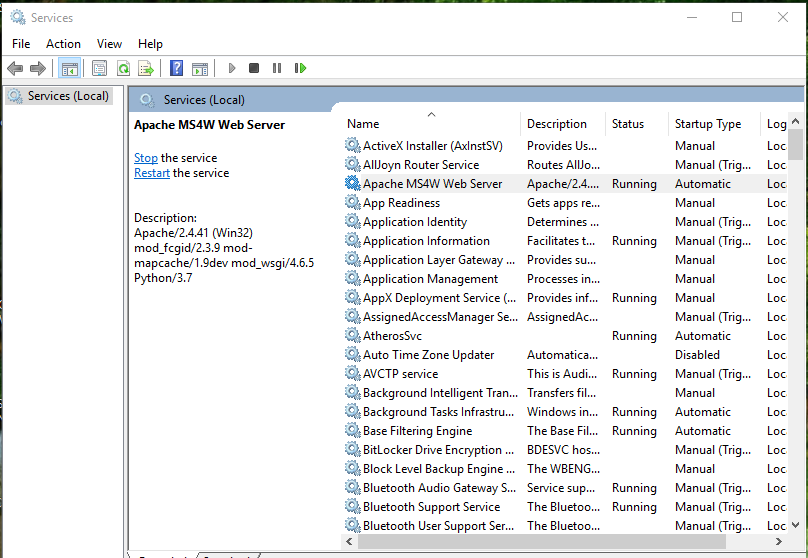
\includegraphics[width=4cm]{figures/1174002/4/8.png}
		\centering
		\caption{Pengaturan Service Apache MS4W Web Server}
    \end{figure}

  \item Jika sudah menemukannya klik 2x
  \item Dan setting seperti berikut
  \hfill\break
    \begin{figure}[H]
		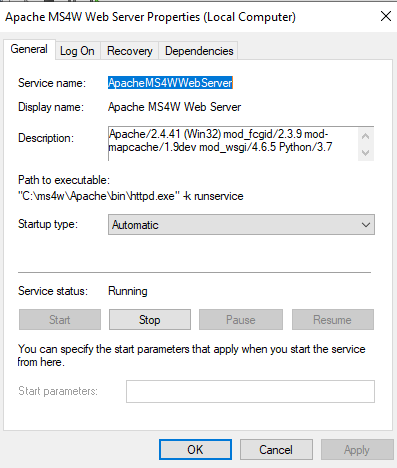
\includegraphics[width=4cm]{figures/1174002/4/9.png}
		\centering
		\caption{Pengaturan Service Apache MS4W Web Server}
    \end{figure}

\end{enumerate}



\subsection{Link Youtube}
\href{https://youtu.be/JQA5rCt7E40}{Klik disini}